%!TEX root = ../main.tex
\section{Augmenting path algorithms}
\subsection{Introduction}
The idea behind the augmenting path algorithms is as follows : 
As long as there is a path from the source to the sink in the residual network, we send flow along this path. And so on until there is no more path from the source to the sink.\newline

A directed path from the source to the sink in the \textit{residual network} is called \textit{augmenting path}. \newline

When an \textit{augmenting path} is found, we send a flow equivalent to the minimum capacity of any edge in the path. We update the \textit{residual network} by decreasing capacities in forward edges and increasing capacities in backward edges. Then we look for a new augmenting path in the new \textit{residual network}. \newline

Here is a graph with its \textit{residual network} after sending 4 units of flow through the \textit{augmenting path} A-C-E-F : \newline

\begin{figure}[!h]
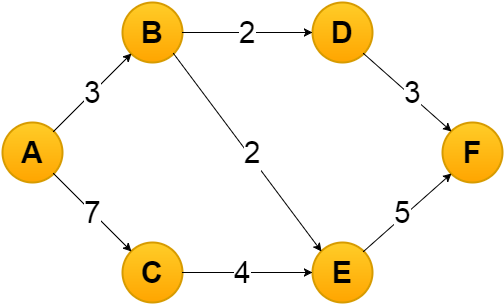
\includegraphics[scale=0.4]{images/graph.png}\hfill
\includegraphics[scale=0.4]{images/graph-residual.png}
\end{figure}
\newpage
The residual network is essential to be able to backtrack. For instance, after sending 4 units of flow through the path A-B-E-F in the graph $G1$, we obtain the graph $G2$. On this graph, it is not possible to find a new path from the source A to the sink F. But on its residual graph $G3$, we can send 2 units of flow through A-C-E-B-D-F to obtain the maximal flow represented in the graph $G4$.


\begin{figure}[h!]
   \begin{minipage}[b]{0.40\linewidth}
      \centering \includegraphics[scale=0.4]{images/graph1a.png}
      \caption{Graph $G1$.}
   \end{minipage}\hfill
   \begin{minipage}[b]{0.48\linewidth}   
      \centering \includegraphics[scale=0.4]{images/graph2.png}
      \caption{Graph $G2$.}
   \end{minipage}\hfill
   \begin{minipage}[b]{0.48\linewidth}   
      \centering \includegraphics[scale=0.4]{images/residualgraph1.png}
      \caption{Residual graph $G3$.}
   \end{minipage}\hfill
   \begin{minipage}[b]{0.48\linewidth}  
      \centering \includegraphics[scale=0.4]{images/graph3.png}
      \caption{Graph $G4$.}
   \end{minipage}
\end{figure}

The pseudo-code of the augmenting path algorithm is given here :

\begin{algorithm}[h]

 \While{$G_f$ contains a directed path from vertex s to vertex t}{
  identify an augmenting path P from vertex s to vertex t\;
  $\delta$ = min\{$c_{ij} : (i,j) \in P$\}\;
  augment $\delta$ units of flow along P and update $G_f$\;
 }
\end{algorithm}

\newpage
\subsection{Ford-Fulkerson and Edmonds-Karp}
There are two main augmenting path algorithms, Ford-Fulkerson (published in 1956) and Edmonds-Karp (published in 1972). They instantiate in their own way the augmenting path algorithm given that the unique difference between both is the way of looking for an \textit{augmenting path} in the \textit{residual network}. \newline

Ford-Fulkerson uses a depth-first search, looking for long paths. The flow is thus sent on a large number of edges but a small quantity. Indeed, a long path have a higher chance to contains at least one edge with a low capacity. \newline

On the other hand, Edmonds-Karp uses a breadth-first search, looking for the shortest path (in terms of number of edges). A bigger quantity of flow is thus sent on a smaller number of edges. \newline


\subsection{Complexities}
The max flow problem, being a problem of complexity class P, can be solved in polynomial time. When the capacities are integers, the remaining time of Ford-Fulkerson is bounded by $O(|E|*|V|*U)$ and Edmonds-Karp by $O(|V|*|E|^2)$, where $|E|$ is the number of edges in the graph, $|V|$ is the number of vertices and $U$ is the maximum capacity of the graph.

\begin{description}
\item[Ford-Fulkerson]{Each augmenting path can be found in $O(|E|)$ thanks to the depth-first search algorithm and in the worst case, the flow will increase by 1. So the time complexity is $O(|E|*|f|)$, $|f|$ being the value of the maximal flow. 

This complexity is expressed in terms of the final result, we can reformulate it. Indeed, the maximal flow cannot be greater than $|V|*U$. The time complexity of Ford-Fulkerson is then $O(|E|*|V|*U)$.

Ford-Fulkerson has a pseudo-polynomial time complexity. Indeed, $O(|E|*|V|*U)$ is polynomial in the numeric value of the input but is exponential in the length of the input. The input takes $log(U)$ bits to represent $U$.}

\item[Edmonds-Karp]{The breadth-first search assures us that after each iteration, the length of the augmenting path can't decrease. We also know that there is a maximum of $|E|$ path of the same length. So we conclude that the length of the augmenting path can stay the same for at most $|E|$ iterations before increasing. 

We know that the length of the augmenting path is between $1$ and $|V|-1$. The length of the augmenting path increase by a least 1 so there is a maximum of $|V|$ possible increases. Thus there are at most $|V|*|E|$ iterations.

We know that each augmenting path can be found in $O(|E|)$. The time complexity of Edmonds-Karp is then $O(|V|*|E|^2)$.}
\end{description}



\section{Preflow-push algorithms}

\subsection{Introduction}

The drawback of the augmenting path algorithms is the operation of sending flow along a path. The time complexity of this operation in the worst case is $O(n)$, where $n$ is the number of vertices in the augmenting path. One example of this  can be seen in the figure \ref{img:bad_augmenting}. With augmenting path algorithms, only one unit of flow can be pushed at a time on the edge $(12, 13)$ in the network. In this case, a better solution is to push directly from the vertice 12, 10 units of flow to the sink. This is the idea behing preflow-push algorithms.

\begin{figure}[H]
\centering
\includegraphics[scale=0.5]{images/bad_augmenting.png}
\caption{Extreme case for augmenting path algorithms.}
\label{img:bad_augmenting}
\end{figure}

The preflow-push algorithms don't push flow on augmenting path, they push flow on individual vertices. Because of this, preflow-push algorithms does not respect the flow conservation constraint. Indeed, these algorithms permit the flow entering a vertex to exceed the flow leaving the vertex. We call this flow a preflow.

\begin{definition}
\label{preflow}
A \textbf{preflow} is a function $x: E \to \mathbb{R}$ that satisfies the capacity constraint and the following relaxation of the flow conservation constraint:
$$\sum\limits_{(j,i) \in E} x_{ji} - \sum\limits_{(i,j) \in E} x_{ij} \geq 0 \text{	for each } i \in V \setminus \{s, t\}.$$
\end{definition}

\begin{definition}
\label{excess}
The \textbf{excess} of each vertex $i \in V$ is 
$$e(i) = \sum\limits_{(j,i) \in E} x_{ji} - \sum\limits_{(i,j) \in E} x_{ij}.$$
\end{definition}

We call a vertex with positive excess as an \textbf{active vertex}. The fact that there are active vertices means that the current solution is not feasible. Thus, the goal of the algorithm is to remove the excess from those vertices. The intuition is to push the flow to the vertex closer to the sink. Each vertex has its own height label which is the distance between the vertex and the sink: the algorithm only push a flow from a vertex to another if the first one is an active vertex and if his height label is greater than the height label of the other vertex. A popular analogy is that we can only push flow downhill. The difference between the two heights label must be one. When we can push a flow from a active vertex to another vertex, we call the edge linking the two an \textbf{admissible edge}. This operation is called a \textbf{push operation}. If such scenario cannot be applied, we need to relabel the height label of the vertex. This operation is called the \textbf{relabel operation}. The algorithm terminates when there is no more active vertex. The pseudo code of this algorithm is given in  Algorithm \ref{pralgo}.


\begin{algorithm}
 preprocess\;
 \While{the network contains an active vertex}{
 select an active vertex $i$\;
 push/relabel($i$)\;
 }
\caption{Generic preflow-push algorithm.}
\label{pralgo}
\end{algorithm}

\begin{algorithm}
 $x\gets 0$\;
 compute height labels $d(i)$\;
 $x_{sj}\gets c_{sj} \text{ for each arc } (s, j) \in E(s)$\;
 $d(s)\gets v$\;
\caption{Preprocess.}
\end{algorithm}

\begin{algorithm}
\If{the network contains an admissible edge $(i, j)$} 
  {push $\delta\gets min\{e(i), r_{ij}\}$ units of flow from $i$ to $j$\;}
\Else
   {replace $d(i)$ by $min\{d(j)+1 : (i, j) \in E(i) \text{ and } r_{ij} > 0 \}$\;}
\caption{Push/Relabel($i$).}
\end{algorithm}

\subsection{Complexity}

To compute the complexity of the generic preflow-push algorithm we need to distinguish three kinds of operations: relabels, saturing pushes, non-saturing pushes.
\begin{itemize}
\item There is a possibility of maximum $|V|^2$ relabel operations. This is because the maximum height is $2*|V| - 1$ and we can decrease the label height at minimum one per operation. We know that there is $|V| - 2$ vertices which can be relabeled (the sink and source vertices can't be relabeled). Then, the maximum number of relabelling is $(2*|V| - 1) * (|V| - 2) \approx |V|^2$.

\item The number of saturing pushes per edge is $O(|V|)$. To make a saturing push on a certain edge again, the label height of the destination vertex must be augmented of 2. Then there is $O(\frac{2*|V| - 1}{2}) \approx O(|V|)$ saturing push per edge: the number of maximum saturing push is $O(|V|*|E|)$.

\item The number of non-saturing pushes is computed with $\phi$, the sum of the height labels of the actives vertices. The relabel increases $\phi$ at maximum $(2*|V| - 1)*(|V|-2)$ (the number of vertices times the maximum height label). The saturing push increase $\phi$ at maximum $(2*|V|-1)*(2*|V|*|E|)$. As $\phi$ must be equals to zero at the end of the algorithm, we need at least $(2*|V|-1)*(|V|-2) + (2*|V|-1)*(2*|V|*|E|) = O(|V|^2*|E|)$ non-saturing push to have $\phi = 0$.
\end{itemize}
We have $O(|V|^2)$ relabel operation, $O(|V|*|E|)$ saturing push and $O(|V|^2*|E|)$ non-saturing push. Thus, the generic preflow algorithm runs in $O(|V|^2) + O(|V|*|E|) + O(|V|^2*|E|) = O(|V|^2 *|E|)$. 

\subsection{Drawbacks}

\subsubsection{The ping-pong effect}

To describe the ping-pong effect, we will execute the preflow push algorithm on the network in Figure \ref{img:pingpong1}.

\begin{figure}[H]
\centering
\includegraphics[scale=0.4]{images/pingpong1.png}
\caption{The initial graph. c is an integer greater than 4.}
\label{img:pingpong1}
\end{figure}

After the preprocess, we push a flow along the path 8-7-6-5-4-3-2-1-t. To be able to do this push, the vertices must be relabeled. We obtain the residual network given in the figure \ref{img:pingpong2} with the corresponding labels for each vertices. The vertex 1 is active. The algorithm relabels it with the height 3. Then, the flow is pushed along the path from the vertex 1 to the vertex 8, and relabel the height labels of the visited vertices. After thoses push and relabel operations, we obtain the residual network described in the figure \ref{img:pingpong3}.

\begin{figure}[H]
\centering
\includegraphics[scale=0.4]{images/pingpong2.png}
\caption{The residual network after some iterations. The only active node is node 1.}
\label{img:pingpong2}
\end{figure}

The algorithm will now select the vertex 8, relabels it to the height label 5 and push the excess flow from 8 to 7. The vertex 7 is selected, his height label modified to 6 and the excess flow is pushed from 7 to 6. The algorithm repeats those operations for each vertices along the path 6-5-4-3-2-1. We obtain now the residual network described in the figue \ref{img:pingpong4}.

\begin{figure}[H]
\centering
\includegraphics[scale=0.4]{images/pingpong3.png}
\caption{The only active node is node 8.}
\label{img:pingpong3}
\end{figure}

We obtain a residual network that look like the residual network in the figure \ref{img:pingpong2}. The only differences are the height label of the bottom vertices. The algorithm will relabel and push the vertices along the path 1-2-3-4-5-6-7-8. We have now the residual network described in the figure \ref{img:pingpong5}.
\begin{figure}[H]
\centering
\includegraphics[scale=0.4]{images/pingpong4.png}
\caption{Node 1 is active again.}
\label{img:pingpong4}
\end{figure}

This round trip between the vertex 1 and the vertex 8 is called the ping-pong effect and is the main drawback of the preflow push algorithms. This flow exchange terminates when the height label of the vertex 8 become greater than the height label of the source.


\begin{figure}[H]
\centering
\includegraphics[scale=0.4]{images/pingpong5.png}
\caption{Node 8 is active again}
\label{img:pingpong5}
\end{figure}
